\documentclass{article}
\usepackage{tikz}
\usepackage{tikzpeople}

\usetikzlibrary{arrows, automata, calc, positioning}
\begin{document}

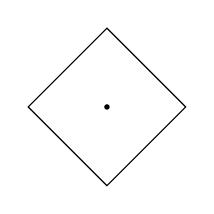
\begin{tikzpicture}
  \draw (1,0) -- (0,1) -- (-1,0) -- (0,-1) -- cycle;
  \fill (0,0) circle (1pt);
\end{tikzpicture}

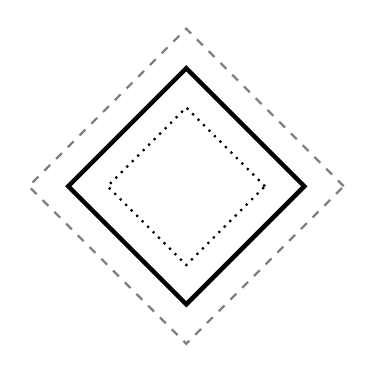
\begin{tikzpicture}
  \draw[thick, dotted] (1,0) -- (0,1) -- (-1,0) -- (0,-1) -- cycle;
  \draw[ultra thick] (0:1.5) -- (90:1.5) -- (180:1.5) -- (270:1.5) -- cycle;
  \draw[dashed, thick, color = gray] (0 r:2) -- (pi/2 r:2) -- (pi r:2) -- (3/2*pi r:2) -- cycle;
\end{tikzpicture}

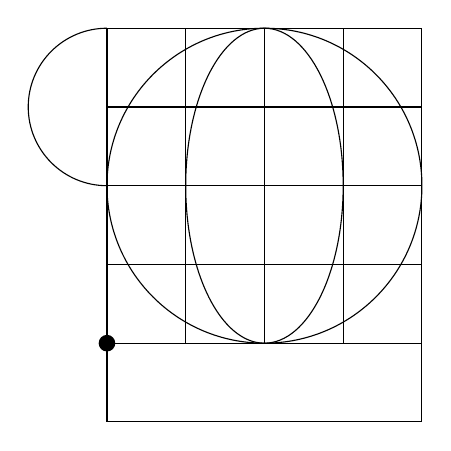
\begin{tikzpicture}
  \draw (0,0) grid (4,4);
  \draw (2,2) circle (2);
  \draw (2,2) circle (1 and 2);
  \draw (0,0) rectangle (4,-1);
  \draw (0,4) arc(90:270:1);
  \fill (0,0) circle (3pt);
\end{tikzpicture}

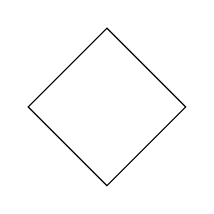
\begin{tikzpicture}
  \coordinate (P0) at (1,0);
  \coordinate (P1) at (0,1);
  \coordinate (P2) at (-1,0);
  \coordinate (P3) at (0,-1);

  \draw (P0) -- (P1) -- (P2) -- (P3) -- cycle;
\end{tikzpicture}

\begin{tikzpicture}
  \tikzstyle{every node} = [draw, shape = circle];

  \node (v0) at (0:0) {$v_0$};
  \node (v1) at (0:2) {$v_1$};
  \node (v2) at (90:2) {$v_2$};
  \node (v3) at (180:2) {$v_3$};
  \node (v4) at (270:2) {$v_4$};

  \draw (v0) -- (v1) (v0) -- (v2) (v0) -- (v3) (v0) -- (v4);
\end{tikzpicture}

% \begin{tikzpicture}
%   \foreach \i in {0,...,3}
%   { \draw ({\i*pi/2} r:1) -- ({(\i+1)*pi/2} r:1); }
% \end{tikzpicture}

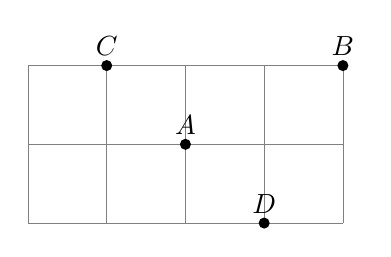
\begin{tikzpicture}
  \draw[help lines] (0,0) grid (4,2);
  \coordinate [label = above: $A$] (A) at (2,1);

  \coordinate [label = above: $B$] (B) at ($2*(A)$);
  \coordinate [label = above: $C$] (C) at ($(A) + (-1,1)$);
  \coordinate [label = above: $D$] (D) at ($(A) - (-1,1)$);

  \fill (A) circle (2pt) (B) circle (2pt) (C) circle (2pt) (D) circle (2pt);
\end{tikzpicture}

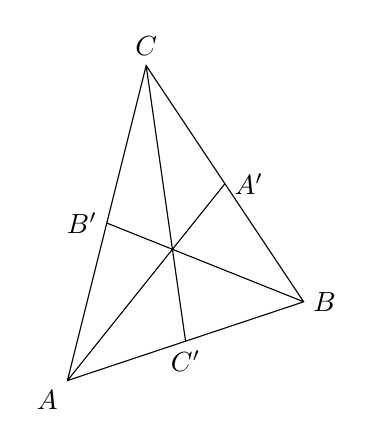
\begin{tikzpicture}
  \coordinate[label=below left:$A$] (A) at (0, 0) ;
  \coordinate[label=right:$B$] (B) at (3, 1) ;
  \coordinate[label=above:$C$] (C) at (1, 4) ;

  \coordinate[label=right:$A'$] (APrime) at ($(B)!0.5!(C)$) ;
  \coordinate[label=left:$B'$] (BPrime) at ($(A)!0.5!(C)$) ;
  \coordinate[label=below:$C'$] (CPrime) at ($(B)!0.5!(A)$) ;

  \draw (A) -- (B) -- (C) -- cycle (A) -- (APrime) (B) -- (BPrime) (C) -- (CPrime);
  
\end{tikzpicture}

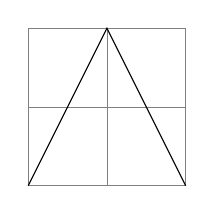
\begin{tikzpicture}
  \draw[help lines] (0,0) grid (2,2);
  \draw let \p1=(0,0), \p2=(1,2), \p3=(2,0) in (\p1) -- (\p2) -- (\p3);
\end{tikzpicture}

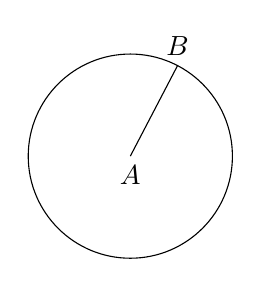
\begin{tikzpicture}
  \coordinate [label=below:$A$] (A) at (0.5,0.75);
  \coordinate [label=above:$B$] (B) at (1.1,1.90);

  \draw (A) -- (B);

  \draw (A) let \p1=($(B) - (A)$) in circle ({veclen(\x1, \y1)});
\end{tikzpicture}

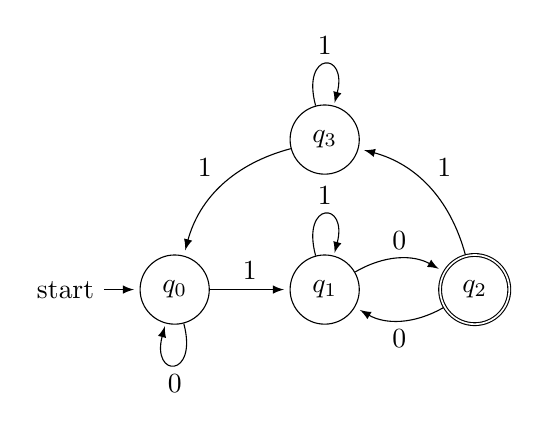
\begin{tikzpicture}[>=latex, shorten >=2pt, node distance = 0.75in, on grid, auto]
  % Vertices of automaton
  \node[state, initial]   (q0)                {$q_0$};
  \node[state]            (q1) [right=of q0]  {$q_1$};
  \node[state, accepting] (q2) [right=of q1]  {$q_2$};
  \node[state]            (q3) [above=of q1]  {$q_3$};

  % Edges of automaton
  \path[->] (q0) edge [loop below]  node {0} (q0)
            (q1) edge [loop above]  node {1} (q1)
            (q3) edge [loop above]  node {1} (q3)
            (q0) edge               node {1} (q1)
            (q1) edge [bend left]   node {0} (q2)
            (q2) edge [bend left]   node {0} (q1)
            (q2) edge [bend right]  node[swap] {1} (q3)
            (q3) edge [bend right]  node[swap] {1} (q0)                        
 ;
\end{tikzpicture}

Use TikZPeople
\begin{tikzpicture}
  \node[alice] at (0,0);
\end{tikzpicture}


\end{document}
%%% Local Variables:
%%% mode: latex
%%% TeX-master: t
%%% End:
